\chapter{Solution Design and Implementation}

For this project we have utilized the following technologies extensively.

\begin{itemize}
  \item NodeJS (Loopback 4, WS and GraphQL)
  \item Angular 7 with Highcharts
  \item Docker
  \item Kubernetes
  \item MySQL
  \item RabbitMQ
\end{itemize}

There are a few terms going forward that need to be defined. Below is an explanation of these terms

\begin{itemize}
  \item \emph{Pod} Is a group of one or more docker containers with shared storage and network running within Kubernetes.
  \item \emph{JWT} stand for JSON Web Token is an open standard \href{https://tools.ietf.org/html/rfc7519}{RFC 7519} for securely transmitting data between 2 places in JSON format. For the purposes of this project we will be using it for user authentication.
\end{itemize}


The project has been split up into a number of microservices to allow for maximum code readability and test-ability. The following microservices have been developed to make up the system.

\begin{itemize}
  \item ws-flare-ui
  \item ws-flare-user-api
  \item ws-flare-projects-api
  \item ws-flare-jobs-api
  \item ws-flare-orchestation-api
  \item ws-flare-cloud-foundry-monitor-api
  \item ws-flare-test-client
  \item ws-flare-cloudfoundry-monitor-client
  \item ws-flare-graphql
  \item ws-flare-gateway
  \item ws-flare-helm-chart
\end{itemize}

\subsection{ws-flare-ui}

This service is written in Angular 7. It holds all the code for displaying the user interface to a user. We also use Highcharts.js as a charting library for displaying results. The user interface is extensively tested using Jest testing framework from FaceBook.

\subsection{ws-flare-user-api}

Holds all user authentication information, such as email, user-name and passwords. For making authentication requests we are using JWT tokens to allow a user to query the system. Without this security any user could utilize the system to attack websites so it is important that we have this layer of security. This service is using MySQL for persisted storage. This service is tested using the mocha testing framework for NodeJS.

\subsection{ws-flare-projects-api}

The system allows users to create projects to logically separate each task. This is more for user convenience and adds to the overall UX aesthetics's of the system. All project and task information is stored within this service. This service uses MySQL as persisted storage. This service is also tested using the mocha testing framework for NodeJS.

\subsection{ws-flare-jobs-api}

This service holds information about currently running jobs. The system allows for running multiple jobs at the same time to allow to be truly embedded into continuous integration environments. This service is using MySQL for persisted storage. This service is tested using the mocha testing framework for NodeJS.

\subsection{ws-flare-orchestation-api}

This service handles the orchestation of jobs. It is listening on a rabbitMQ message queue for requests to start new jobs. Once it has received a new request it will calculate how many docker containers it needs to spin up to achieve the requested websocket load. It will then instruct Kubernetes to start the required amount of pods that it needs to start the stress test. It will also instruct kubernetes to start a pod designed specifically for monitoring Cloud Foundry applications. Once all pods have been started, this service will instruct all pods to start the test and for the Cloud Foundry monitor to start monitoring the specified applications. This service has no long term persisted storage mechanism and is testing using the mocha test framework for NodeJS.

\subsection{ws-flare-cloud-foundry-monitor-api}

This service stores information related to running applications on Cloud Foundry, such as memory and CPU at a particular point in time. This service is using MySQL for persisted storage. This service is tested using the mocha testing framework for NodeJS.

\subsection{ws-flare-test-client}

This is an application that can be spun up as a Kubernetes pod. The goal of this application is to simulate a number of websocket connections. A limit of 1000 connections per pod has been specified. For example if we have a test that requires a simulation of 5046 users then 6 ws-flare-test-client pods will be created. Five of those will simulate 1000 connections and the sixth will simulate 46 connections. Together they will simulate the full 5046 connections. For each of the connections established the connection information will be stored within the ws-flare-jobs-api service. The service will contain information on how many connections were successfully established, how many connections have dropped, and how many connections have not connected. We will also store the amount of time or latency it tool to connect to the websocket server. Once the stress test has completed this application will instruct Kubernetes to delete itself. Kubernetes will then proceed to remove the pod. This service has no long term persisted storage mechanism and is testing using the mocha test framework for NodeJS.

\subsection{ws-flare-cloudfoundry-monitor-client}

This is another application that is spun up as a Kubernetes pod. Once it is created it will immediately attempt to connect to the specified Cloud Foundry instance. There it will attempt to find the applications that the user requested to monitor. Once the correct applications have been found this application will send a message back to ws-flare-orchestation-api over a rabbitMQ message queue informing it that it has found the correct applications and is ready to start monitoring. The application will then wait for the orchestration API to create the necessary clients to simulate the Websockets. While the test is in progress the application will actively communicate with the Cloud Foundry instance to interrogate it for applications statistics such as memory and CPU usage. It will also get information from each instance of the application deployed on cloud foundry. Once all tests have completed this application will then shut itself down by instructing kubernetes to kill itself. Kubernetes will then remove the pod. This service has no long term persisted storage mechanism and is testing using the mocha test framework for NodeJS.

\subsection{ws-flare-graphql}

We chose to integrate GraphQL into this architecture due to its ability to easily query multiple services at the same time in one request. Due to the need to present results to the user with minimal latency we felt that this made sense, and very easy to integrate into Angular 7 using apollo-client. 

\subsection{ws-flare-gateway}

This is the API gateway to allow the user interface to communicate with the system. Using an API gateway provides a number of benefits, as everything is served through one endpoint or ip address. Currently the gateway has routes only the GraphQL server and the user interface server. The routes are outlined below

\begin{itemize}
  \item / routes to ws-flare-ui
  \item /graphql routes to ws-flare-graphql
\end{itemize}

The API gateway also provides a layer of security as the only way a user can interact with the system is through those 2 routes. It cannot communicate with any of the underlying services. The underlying technology of this gateway is an nginx server.

\subsection{ws-flare-helm-chart}

This is the helm chart for the entire application. Helm is the package manager for Kubernetes. With helm we can define our entire infrastructure as code. This also provides anyone with a Kubernetes cluster to install the application with one single command

\begin{minted}{bash}
helm install .
\end{minted}

Kubernetes will then work out all the routing between services using its internal DNS server. This makes Kubernetes a very attractive solution for distributing applications, and one of the main reasons Kubernetes was chosen for this project.

\subsection{Utilizing Kubernetes API to test at scale}

Stress testing as the name suggests puts a lot of stress on resources. Not only is this true for the system that is being tested, it is also true for the system performing the test. To eliminate resource drain on the system that is performing the test we need to be easily able to scale the test out for maximum throughput. Using a simple NodeJS script on a 16GB Memory intel core I7 labtop the maximum websockets that could be tested was peaking at around 10000 simultaneous websockets. After this amount it was observed that connections would either drop randomly or not connect at all to a websocket server. 

\begin{minted}{javascript}
var WebSocket = require('ws');

for (let i = 0; i < 100000; i++) {
    var ws = new WebSocket('ws://localhost:9002');

    ws.on('open', function open() {
        console.log('Opened socket ' + i);
        ws.send('PING');
    });

    ws.on('error', () => {
        console.log('Got error');
    });
}
\end{minted}

To maximize the number of websockets we can simulate we need a scalable system. This is the reason why Kubernetes was chosen for this project. With Kubernetes we can easily create new pods to perform the simulations. Kubernetes has a powerful rest API which we can perform a POST request on, passing it the required information it needs to create a new pod. The request looks like the example below.

\begin{minted}{typescript}
kubernetesClient
  .api
  .v1
  .namespaces('default')
  .pod
  .post({
    body: {
      kind: "Pod",
      apiVersion: "v1",
      metadata: {
        labels: {
          app: 'ws-flare-test-client'
        },
        name: 'ws-flare-test-client-abc1'
      },
      spec: {
        containers: [
          {
            name: 'ws-flare-test-client-abc1',
            image: 'wsflare/ws-flare-test-client',
            env: [],
            resources: {
              requests: {
                cpu: '100m'
              }
            }
          },
        ]
      }
    }
  });
  
\end{minted}

The above script will request that Kubernetes create a new Pod using the ws-flare-test-client docker container. We can also pass environment variables to this Pod. Using this API we can also specify how much CPU this pod is assigned. The above expression of 100m means that this pod will have one hundred millicpu. So if 1000m is the equivalent of one CPU then we can say that this Pod will be assigned one tenth of the avilable CPU cycles. From testing the application this is a good enough amount of CPU cycles to simulate 1000 websockets. 

If we consider that making the above request to Kubernetes will yield us one Pod which can simulate 1000 websockets, we can now start to think that if we make 10 requests and are given ten Pods, we can now simulate 10,000 websockets.

There are a number of options for obtaining a kubernetes cluster. Kubernetes can be deployed on an AWS Compute cluster using Amazons web-tools. Pivotal also has its own flavour of Kubernetes in the form of Pivotals Container Service (PKS). However in practive and while working on this project it was found that Google Kubernetes Engine (GKE) was one of the easiest kubernetes clusters to setup. It should also be noted that all of the above are paid services, and can become expensive depending on how much resources are assigned to a cluster. 

To setup a new cluster on GKE here are a few guidelines. The following assumes that you already have setup a GKE account setup.

\begin{figure}[!h]
  \centering
    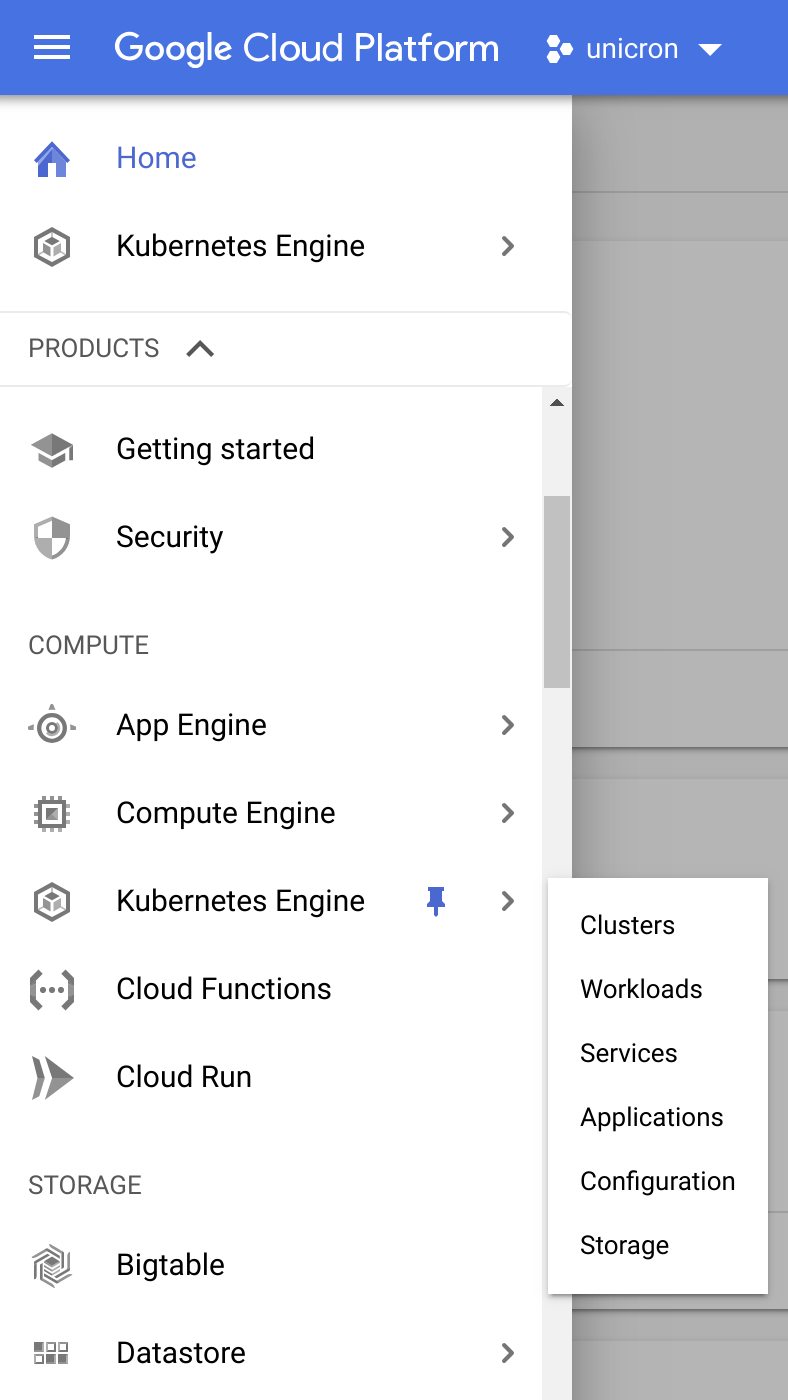
\includegraphics[width=0.5\textwidth]{figures/gke-setup-1.png}
    \caption{Select Kubernetes Engine then select Clusters}
    \label{fig:https-handshake}
\end{figure}

\FloatBarrier

This will bring you into the kubernetes engine screen where you can then create your own cluster from scratch.

\begin{figure}[!h]
  \centering
    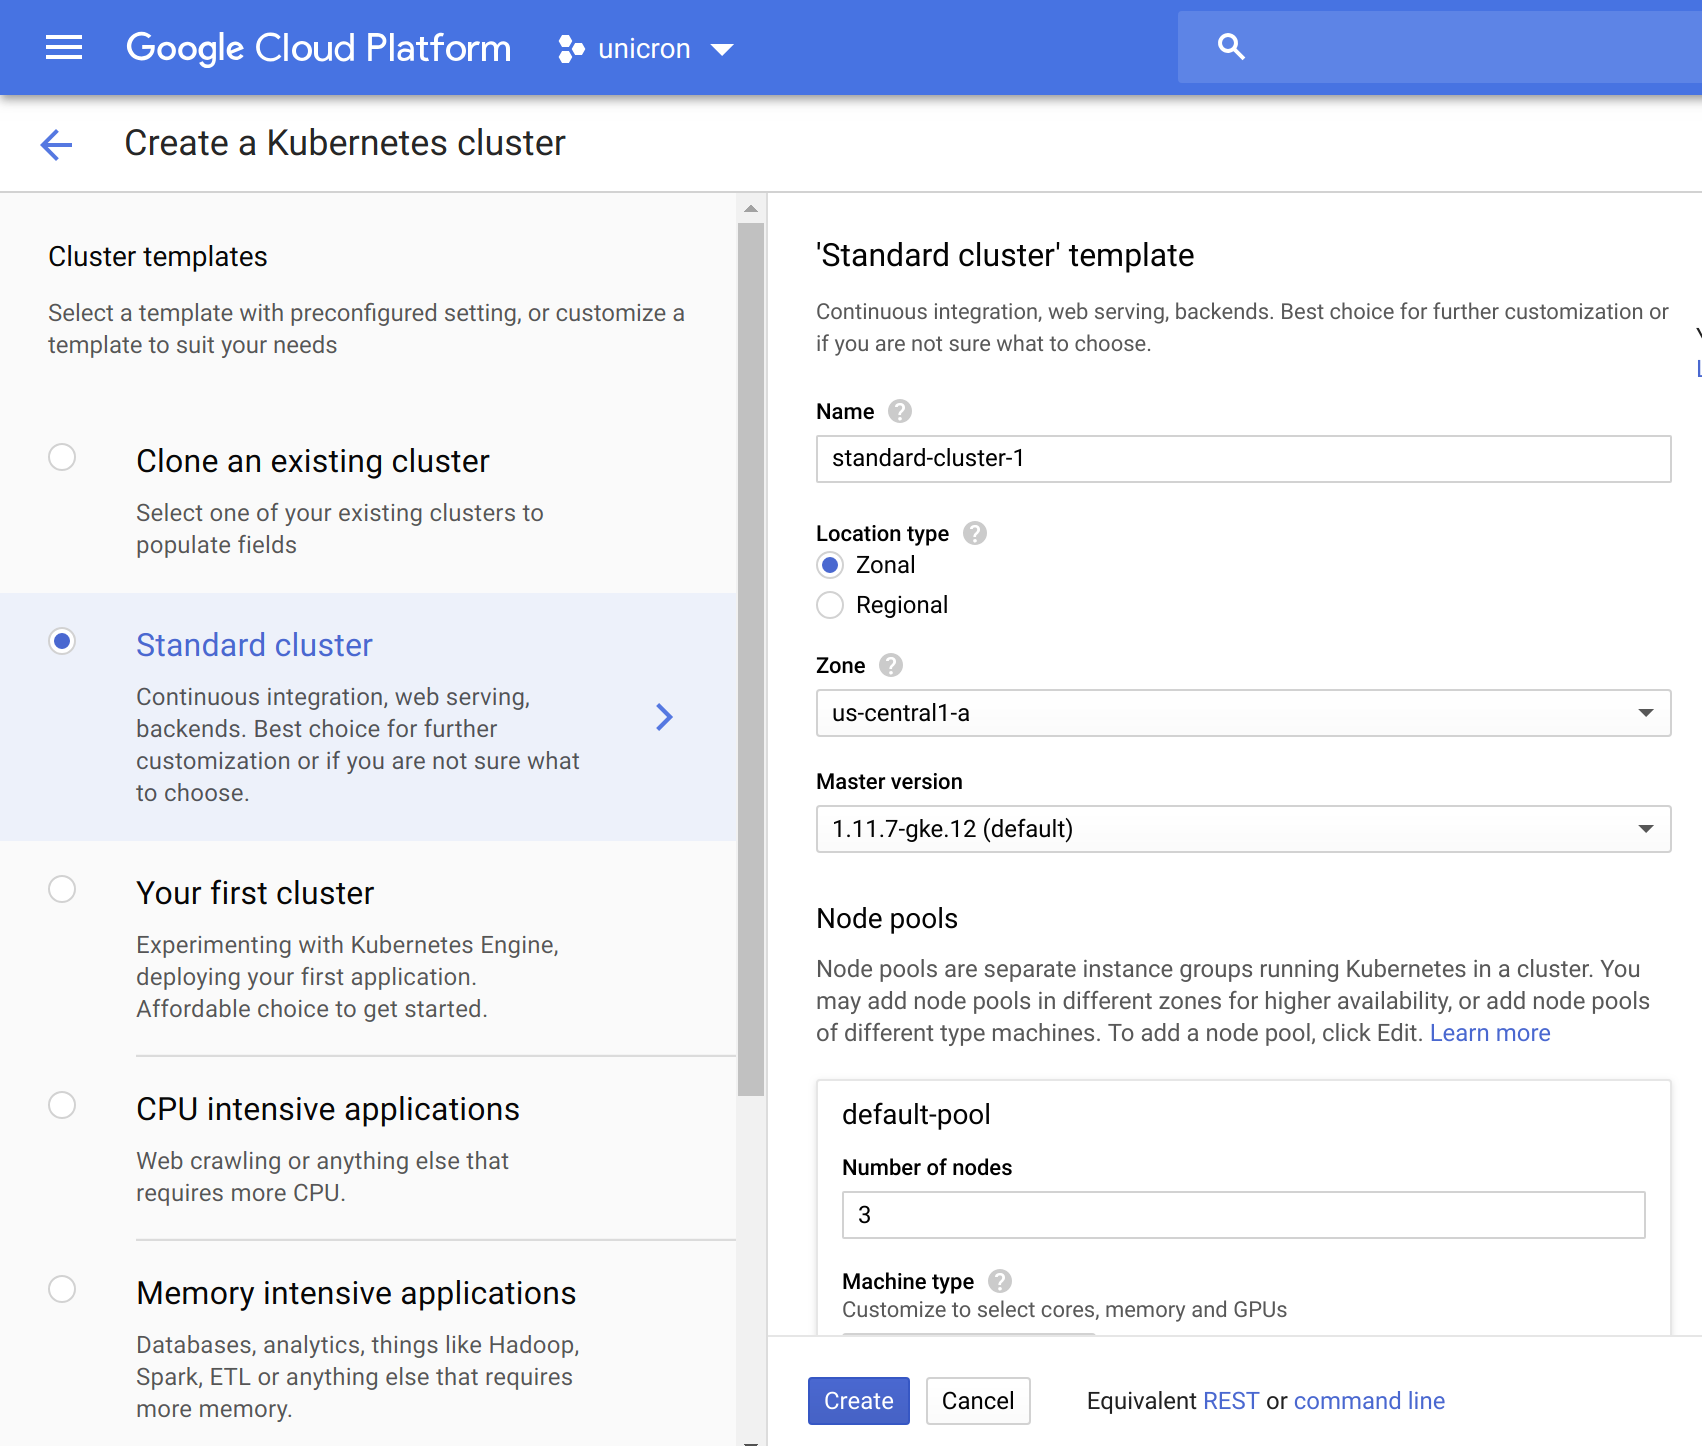
\includegraphics[width=0.8\textwidth]{figures/gke-setup-2.png}
    \caption{Select the resources to assign to this cluster}
    \label{fig:https-handshake}
\end{figure}

\FloatBarrier

Once you have selected your desired cluster resources, click Create and in a few minutes your cluster should be created. Once the cluster is setup you will be given the opportunity to connect to it. 

\begin{figure}[!h]
  \centering
    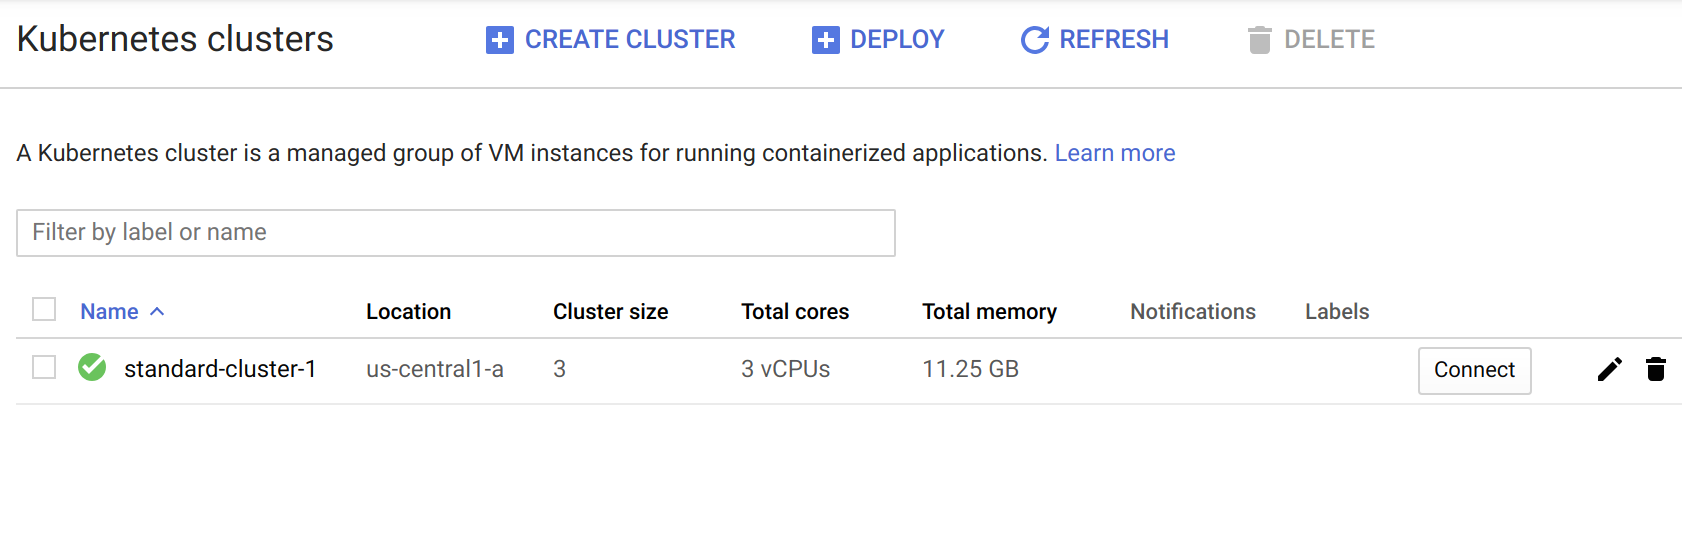
\includegraphics[width=0.8\textwidth]{figures/gke-setup-3.png}
    \caption{Click the connect button to get instructions on how to connect}
    \label{fig:https-handshake}
\end{figure}

\FloatBarrier

After clicking connect you will be given a command that you can run on your machine. Before running this command you will need to install the Google Cloud SDK tools. There is a quickstart guide available
\href{https://cloud.google.com/sdk/docs/quickstart-linux}{here}. Once you have installed the SDK tools then use the command that you have been given from the GKE console and you should be able to connect.